\begin{figure}[h!]
\centering
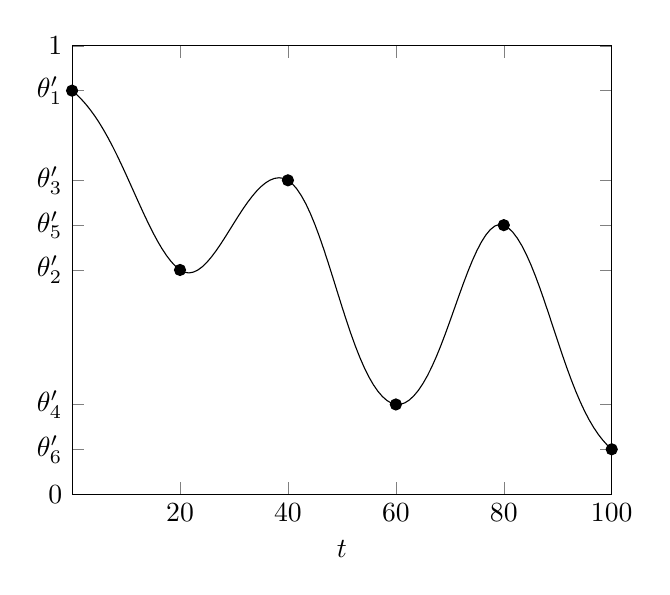
\begin{tikzpicture}
\begin{axis}[xtick={20, 40,...,100}, ytick={0, 0.1, 0.2, 0.5, 0.6, 0.7, 0.9, 1}, yticklabels={0, $\theta_6'$, $\theta_4'$, $\theta_2'$, $\theta_5'$, $\theta_3'$, $\theta_1'$, 1}, xmin=0, xmax=100,  ymin=0, ymax=1, xlabel = $t$]

\addplot[domain=0:20] {1/(1+e^(-((2*((x-0)/(20-0))^3 - 3*((x-0)/(20-0))^2 + 1)*(2.2) + (((x-0)/(20-0))^3 - 2*((x-0)/(20-0))^2+((x-0)/(20-0)))*(0-(2.2)) + (-2*((x-0)/(20-0))^3+3*((x-0)/(20-0))^2)*(0) + (((x-0)/(20-0))^3-((x-0)/(20-0))^2)*1/2*((0-2.2) + (0.8473-0)) )))};
\addplot[domain=20:40] {1/(1+e^(-((2*((x-20)/(40-20))^3 - 3*((x-20)/(40-20))^2 + 1)*0 + (((x-20)/(40-20))^3 - 2*((x-20)/(40-20))^2+((x-20)/(40-20)))*1/2*( (0.8473-0) + (0-(2.2)))+ (-2*((x-20)/(40-20))^3+3*((x-20)/(40-20))^2)*(0.8473) + (((x-20)/(40-20))^3-((x-20)/(40-20))^2)*1/2*((0.8473-0) + (-(1.3863)-0.8473)) )))};
\addplot[domain=40:60] {1/(1+e^(-((2*((x-40)/(60-40))^3 - 3*((x-40)/(60-40))^2 + 1)*0.8473 + (((x-40)/(60-40))^3 - 2*((x-40)/(60-40))^2+((x-40)/(60-40)))*1/2*( (-(1.3863)-0.8473) + (0.8473-0))+ (-2*((x-40)/(60-40))^3+3*((x-40)/(60-40))^2)*(-(1.3863)) + (((x-40)/(60-40))^3-((x-40)/(60-40))^2)*1/2*((-(1.3863)-0.8473) + (0.4054--(1.3863))) )))};
\addplot[domain=60:80] {1/(1+e^(-((2*((x-60)/(80-60))^3 - 3*((x-60)/(80-60))^2 + 1)*-(1.3863) + (((x-60)/(80-60))^3 - 2*((x-60)/(80-60))^2+((x-60)/(80-60)))*1/2*( (0.4054--(1.3863)) + (-(1.3863)-0.8473))+ (-2*((x-60)/(80-60))^3+3*((x-60)/(80-60))^2)*(0.4054) + (((x-60)/(80-60))^3-((x-60)/(80-60))^2)*1/2*((0.4054--(1.3863)) + (-2.1972-0.4054)) )))};
\addplot[domain=80:100] {1/(1+e^(-((2*((x-80)/(100-80))^3 - 3*((x-80)/(100-80))^2 + 1)*0.4054 + (((x-80)/(100-80))^3 - 2*((x-80)/(100-80))^2+((x-80)/(100-80)))*1/2*( (-2.1972-0.4054) + (0.4054--(1.3863)))+ (-2*((x-80)/(100-80))^3+3*((x-80)/(100-80))^2)*(-2.1972) + (((x-80)/(100-80))^3-((x-80)/(100-80))^2)*1/2*((-2.1972-0.4054) + (0.2-2.1972)) )))};
\addplot[mark=*] coordinates {(0,0.9)};
\addplot[mark=*] coordinates {(20,0.5)};
\addplot[mark=*] coordinates {(40,0.7)};
\addplot[mark=*] coordinates {(60,0.2)};
\addplot[mark=*] coordinates {(100,0.1)};
\addplot[mark=*] coordinates {(80,0.6)};
\end{axis}
\end{tikzpicture}
\caption{Example for sigmoid transformed spline $f_{j,A}(\theta; t) = \sigma(S(\theta; t))$}
\end{figure}